\section{Background}

\subsection{Imperfect Information Games}

Imperfect information game is a term from game theory describing games, where information is not fully available to all participants. Classical examples are card games where only you know your hand, like poker.


\subsection{Reinforcement Learning}

\begin{figure}
	\centering
	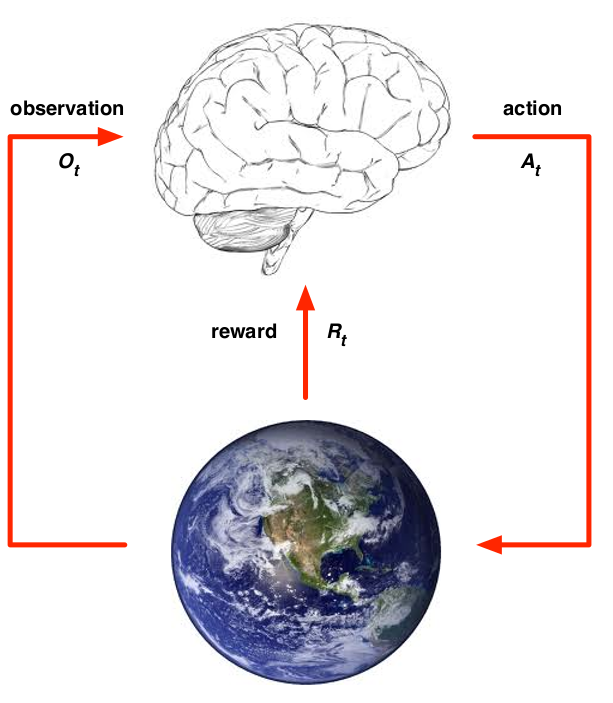
\includegraphics[width=0.7\textwidth]{image/rl_agent_environment}
	\label{img:rl_agent}
	\caption{Agent and Environment\cite{pres:rl_learn}}
\end{figure}



\subsection{Deep Learning}\label{sec:deep_learn}


\subsection{Glossary}

